\documentclass[11pt]{article}
\usepackage[textwidth=18.0cm, textheight=23.0cm, top=2.0cm]{geometry}
\usepackage{pst-all}
\usepackage{amssymb}
\usepackage{tikz}
\usepackage{underscore}\begin{document}
\pagestyle{empty}


ClassName: \underline{\textbf{Class_10.2bp-35}}
\par
BinSize: \underline{\textbf{100 × 100}}
\par
ReduceSize: \underline{\textbf{100 × 100}}
\par
TypeNum: \underline{\textbf{80}}
\par
Num: \underline{\textbf{80}}
\par
OutS: \underline{\textbf{130000}}
\par
InS: \underline{\textbf{122105}}
\par
Rate: \underline{\textbf{0.939}}
\par
UB: \underline{\textbf{13}}
\par
LB0: \underline{\textbf{13}}
\par
LB: \underline{\textbf{13}}
\par
LBWithCut: \underline{\textbf{13}}
\par
NodeCut: \underline{\textbf{0}}
\par
ExtendedNodeCnt: \underline{\textbf{1}}
\par
GenNodeCnt: \underline{\textbf{1}}
\par
PrimalNode: \underline{\textbf{0}}
\par
ColumnCount: \underline{\textbf{13}}
\par
TotalCutCount: \underline{\textbf{0}}
\par
RootCutCount: \underline{\textbf{0}}
\par
LPSolverCnt: \underline{\textbf{1}}
\par
PricingSolverCnt: \underline{\textbf{0}}
\par
BranchAndBoundNum: \underline{\textbf{1}}
\par
isOpt: \underline{\textbf{true}}
\par
TimeOnInitSolution: \underline{\textbf{1.850 s}}
\par
TimeOnPrimal: \underline{\textbf{0.000 s}}
\par
TimeOnPricing: \underline{\textbf{0.000 s}}
\par
TimeOnRmp: \underline{\textbf{0.062 s}}
\par
TotalTime: \underline{\textbf{1.975 s}}
\par
\newpage


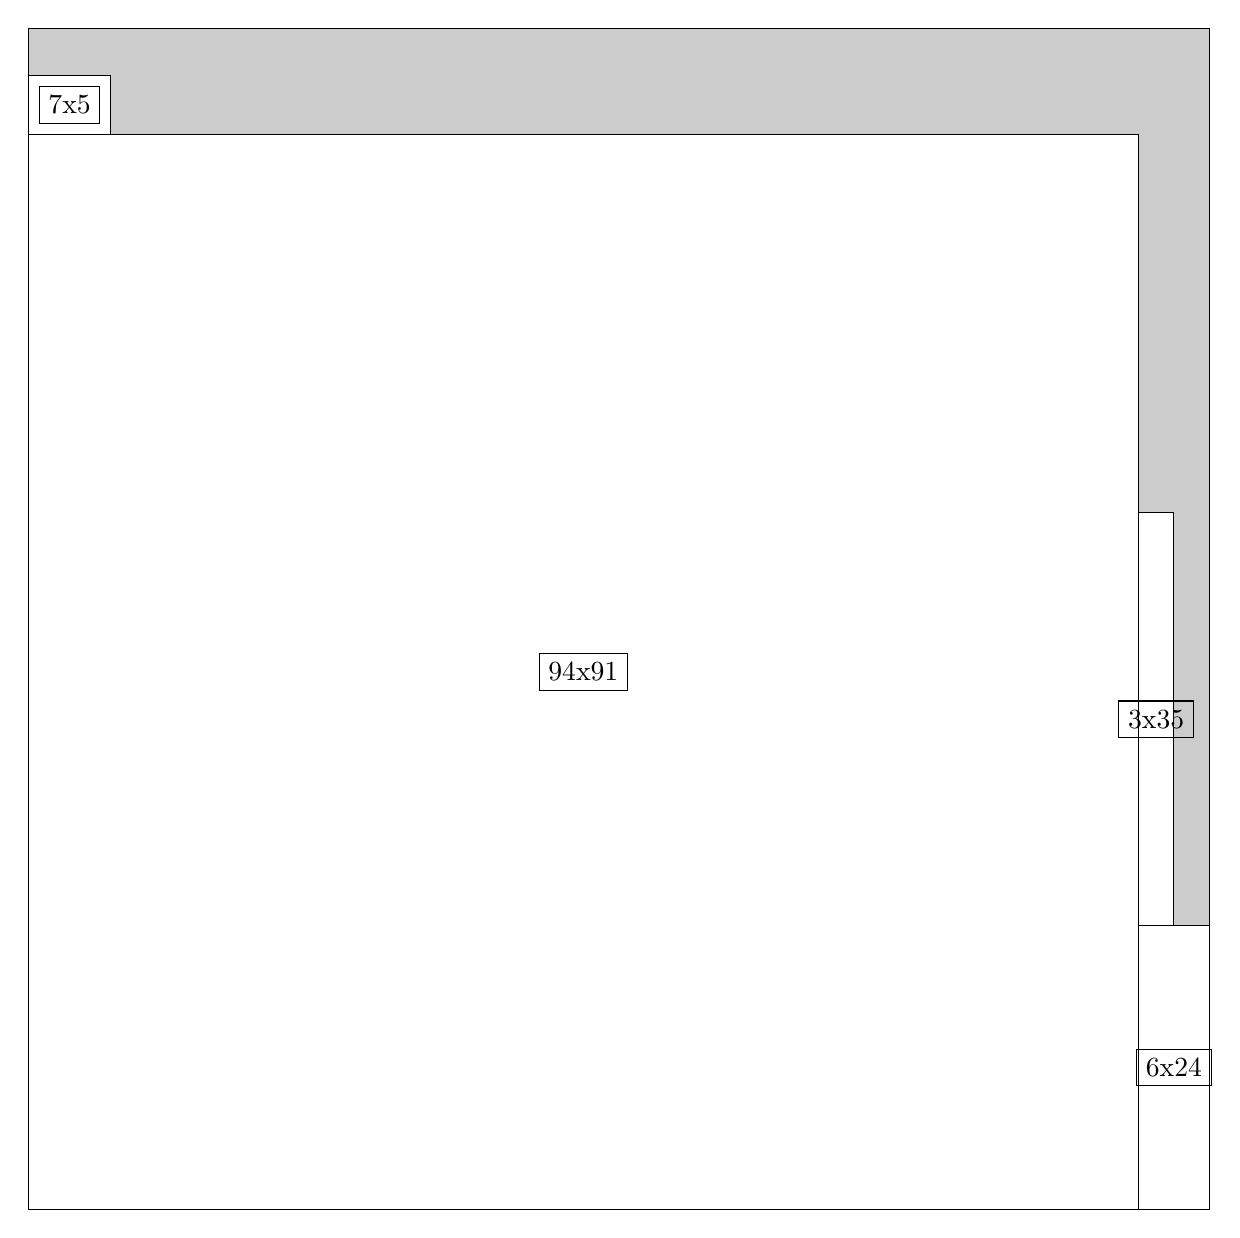
\begin{tikzpicture}[shorten >=1pt,scale=1.0,every node/.style={scale=1.0},->]
\tikzstyle{vertex}=[circle,fill=black!25,minimum size=14pt,inner sep=0pt]
\filldraw[fill=gray!40!white, draw=black] (0,0) rectangle (15.0,15.0);
\foreach \name/\x/\y/\w/\h in {94x91/0.0/0.0/14.1/13.65,6x24/14.1/0.0/0.8999999999999999/3.5999999999999996,3x35/14.1/3.5999999999999996/0.44999999999999996/5.25,7x5/0.0/13.65/1.05/0.75}
\filldraw[fill=white!40!white, draw=black] (\x,\y) rectangle node[draw] (\name) {\name} ++(\w,\h);
\end{tikzpicture}


w =94 , h =91 , x =0 , y =0 , v =8554
\par
w =6 , h =24 , x =94 , y =0 , v =144
\par
w =3 , h =35 , x =94 , y =24 , v =105
\par
w =7 , h =5 , x =0 , y =91 , v =35
\par
\newpage


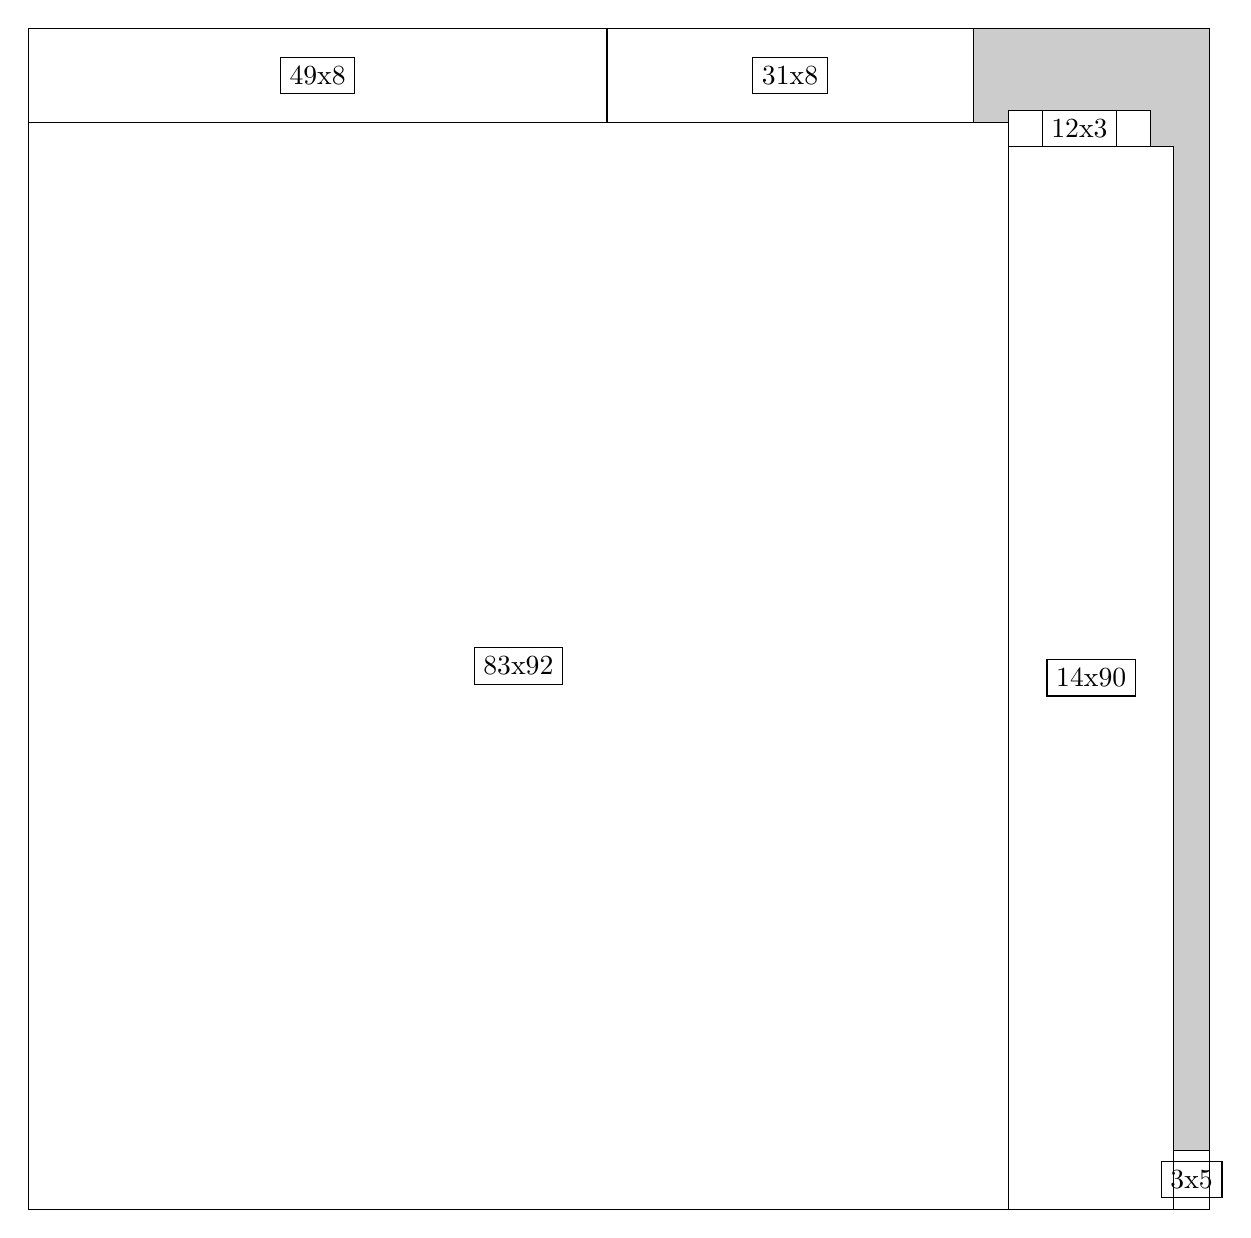
\begin{tikzpicture}[shorten >=1pt,scale=1.0,every node/.style={scale=1.0},->]
\tikzstyle{vertex}=[circle,fill=black!25,minimum size=14pt,inner sep=0pt]
\filldraw[fill=gray!40!white, draw=black] (0,0) rectangle (15.0,15.0);
\foreach \name/\x/\y/\w/\h in {83x92/0.0/0.0/12.45/13.799999999999999,14x90/12.45/0.0/2.1/13.5,49x8/0.0/13.799999999999999/7.35/1.2,31x8/7.35/13.799999999999999/4.6499999999999995/1.2,12x3/12.45/13.5/1.7999999999999998/0.44999999999999996,3x5/14.549999999999999/0.0/0.44999999999999996/0.75}
\filldraw[fill=white!40!white, draw=black] (\x,\y) rectangle node[draw] (\name) {\name} ++(\w,\h);
\end{tikzpicture}


w =83 , h =92 , x =0 , y =0 , v =7636
\par
w =14 , h =90 , x =83 , y =0 , v =1260
\par
w =49 , h =8 , x =0 , y =92 , v =392
\par
w =31 , h =8 , x =49 , y =92 , v =248
\par
w =12 , h =3 , x =83 , y =90 , v =36
\par
w =3 , h =5 , x =97 , y =0 , v =15
\par
\newpage


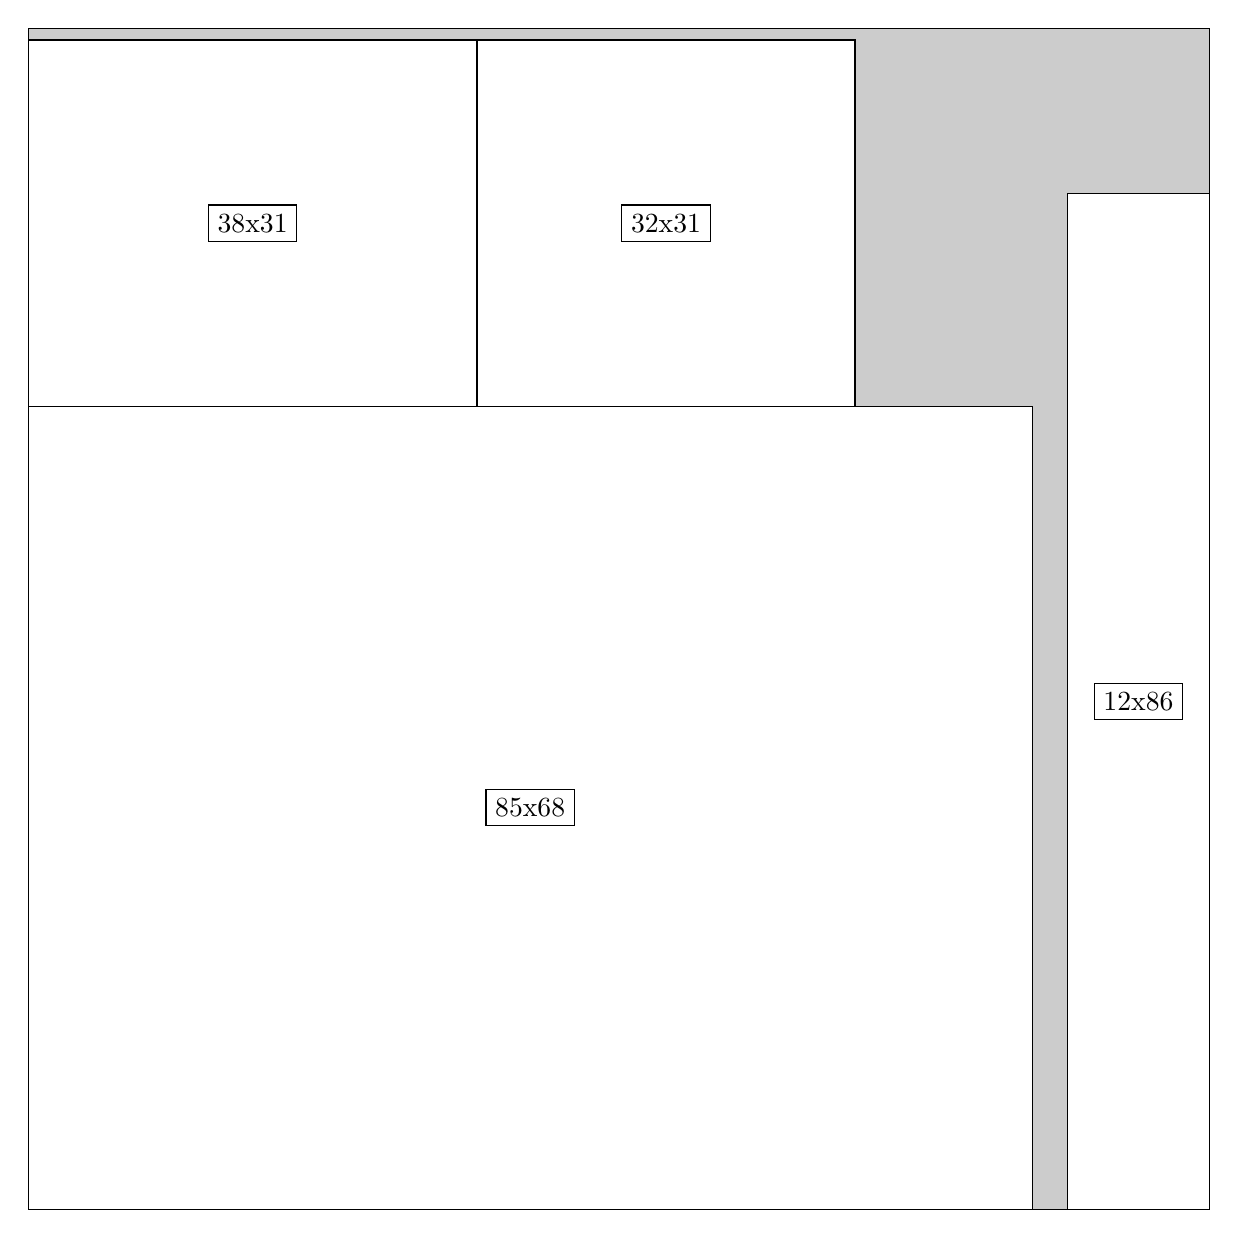
\begin{tikzpicture}[shorten >=1pt,scale=1.0,every node/.style={scale=1.0},->]
\tikzstyle{vertex}=[circle,fill=black!25,minimum size=14pt,inner sep=0pt]
\filldraw[fill=gray!40!white, draw=black] (0,0) rectangle (15.0,15.0);
\foreach \name/\x/\y/\w/\h in {85x68/0.0/0.0/12.75/10.2,38x31/0.0/10.2/5.7/4.6499999999999995,12x86/13.2/0.0/1.7999999999999998/12.9,32x31/5.7/10.2/4.8/4.6499999999999995}
\filldraw[fill=white!40!white, draw=black] (\x,\y) rectangle node[draw] (\name) {\name} ++(\w,\h);
\end{tikzpicture}


w =85 , h =68 , x =0 , y =0 , v =5780
\par
w =38 , h =31 , x =0 , y =68 , v =1178
\par
w =12 , h =86 , x =88 , y =0 , v =1032
\par
w =32 , h =31 , x =38 , y =68 , v =992
\par
\newpage


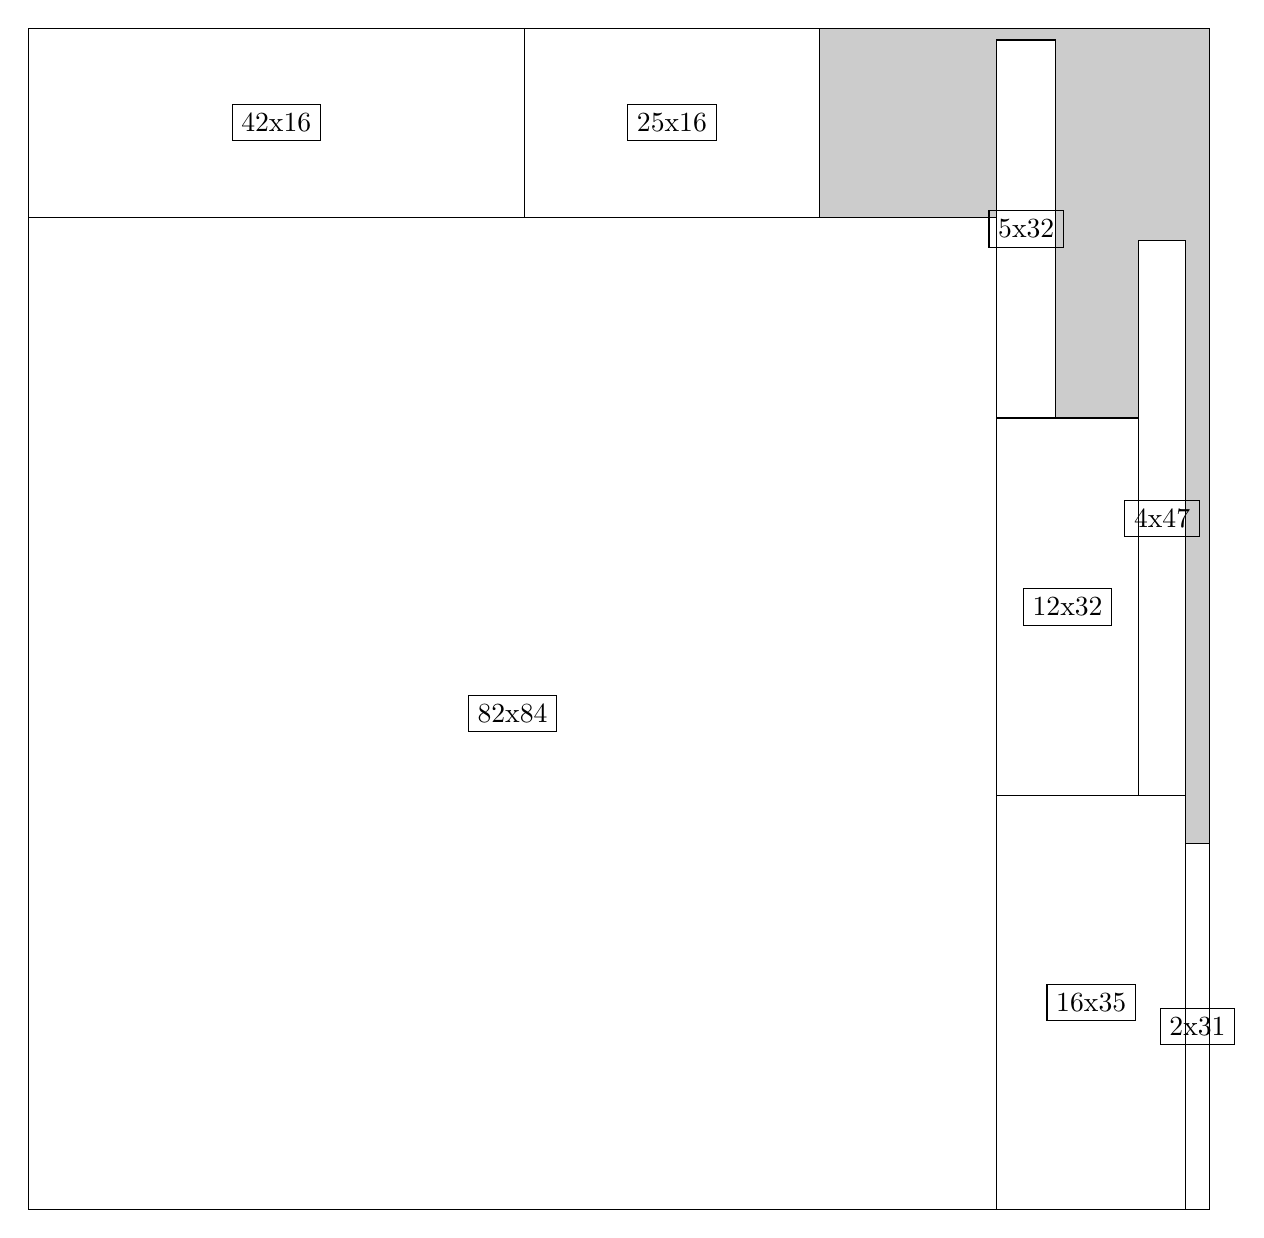
\begin{tikzpicture}[shorten >=1pt,scale=1.0,every node/.style={scale=1.0},->]
\tikzstyle{vertex}=[circle,fill=black!25,minimum size=14pt,inner sep=0pt]
\filldraw[fill=gray!40!white, draw=black] (0,0) rectangle (15.0,15.0);
\foreach \name/\x/\y/\w/\h in {82x84/0.0/0.0/12.299999999999999/12.6,42x16/0.0/12.6/6.3/2.4,16x35/12.299999999999999/0.0/2.4/5.25,25x16/6.3/12.6/3.75/2.4,12x32/12.299999999999999/5.25/1.7999999999999998/4.8,4x47/14.1/5.25/0.6/7.05,5x32/12.299999999999999/10.049999999999999/0.75/4.8,2x31/14.7/0.0/0.3/4.6499999999999995}
\filldraw[fill=white!40!white, draw=black] (\x,\y) rectangle node[draw] (\name) {\name} ++(\w,\h);
\end{tikzpicture}


w =82 , h =84 , x =0 , y =0 , v =6888
\par
w =42 , h =16 , x =0 , y =84 , v =672
\par
w =16 , h =35 , x =82 , y =0 , v =560
\par
w =25 , h =16 , x =42 , y =84 , v =400
\par
w =12 , h =32 , x =82 , y =35 , v =384
\par
w =4 , h =47 , x =94 , y =35 , v =188
\par
w =5 , h =32 , x =82 , y =67 , v =160
\par
w =2 , h =31 , x =98 , y =0 , v =62
\par
\newpage


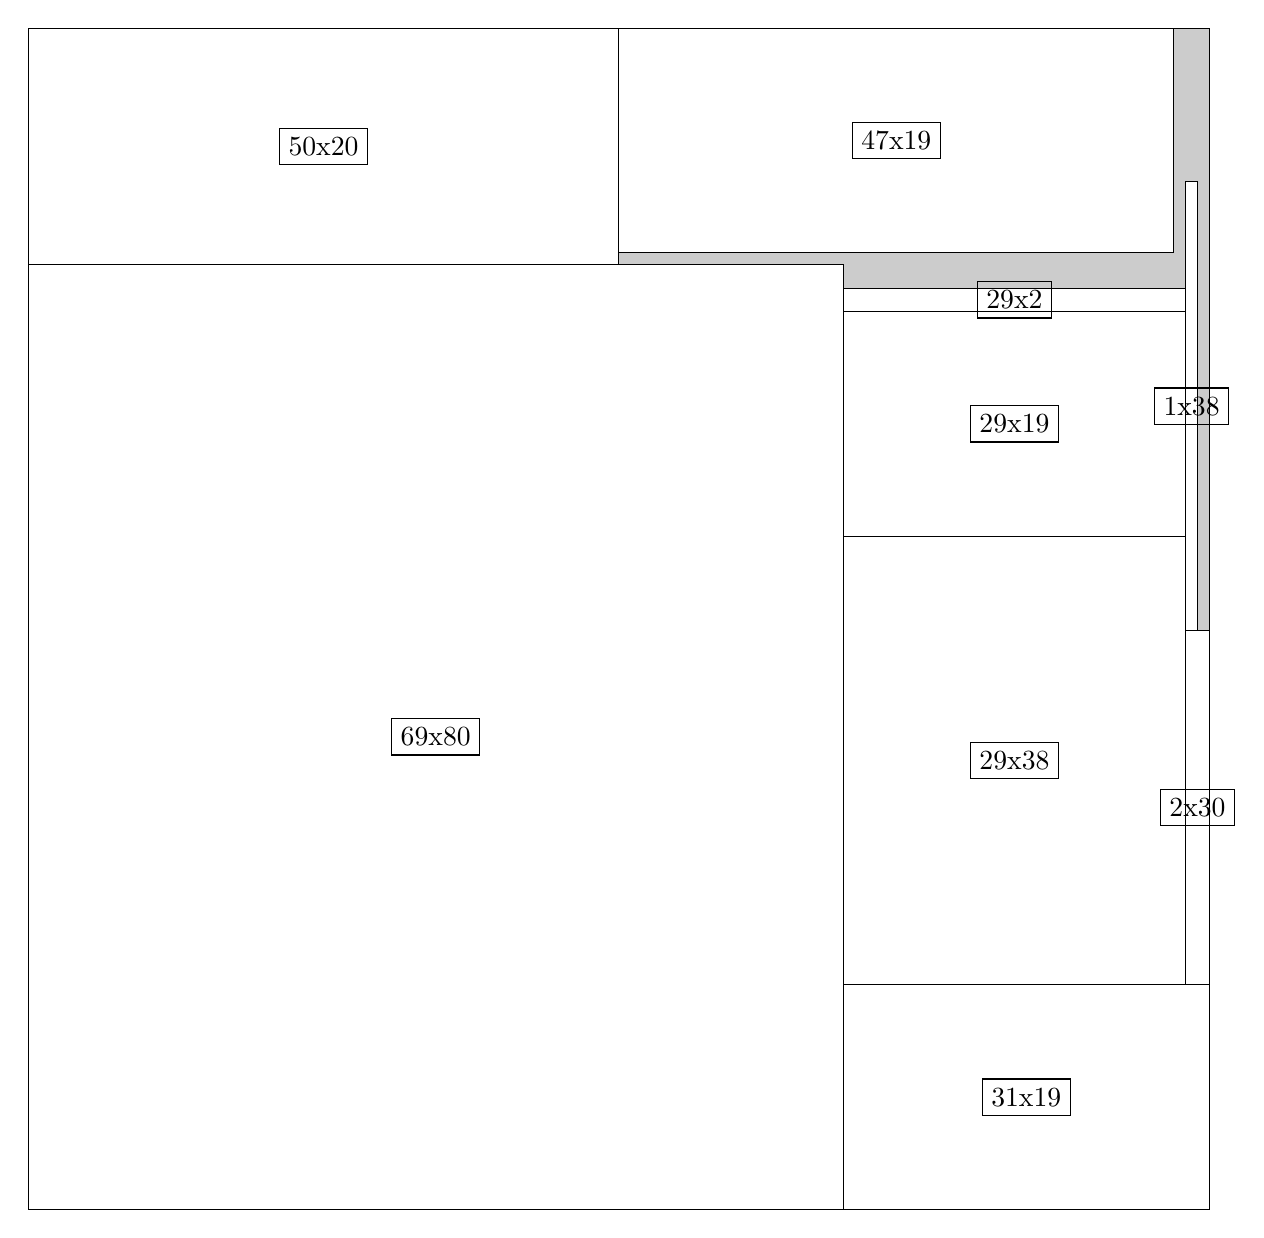
\begin{tikzpicture}[shorten >=1pt,scale=1.0,every node/.style={scale=1.0},->]
\tikzstyle{vertex}=[circle,fill=black!25,minimum size=14pt,inner sep=0pt]
\filldraw[fill=gray!40!white, draw=black] (0,0) rectangle (15.0,15.0);
\foreach \name/\x/\y/\w/\h in {69x80/0.0/0.0/10.35/12.0,29x38/10.35/2.85/4.35/5.7,50x20/0.0/12.0/7.5/3.0,47x19/7.5/12.15/7.05/2.85,31x19/10.35/0.0/4.6499999999999995/2.85,29x19/10.35/8.549999999999999/4.35/2.85,2x30/14.7/2.85/0.3/4.5,29x2/10.35/11.4/4.35/0.3,1x38/14.7/7.35/0.15/5.7}
\filldraw[fill=white!40!white, draw=black] (\x,\y) rectangle node[draw] (\name) {\name} ++(\w,\h);
\end{tikzpicture}


w =69 , h =80 , x =0 , y =0 , v =5520
\par
w =29 , h =38 , x =69 , y =19 , v =1102
\par
w =50 , h =20 , x =0 , y =80 , v =1000
\par
w =47 , h =19 , x =50 , y =81 , v =893
\par
w =31 , h =19 , x =69 , y =0 , v =589
\par
w =29 , h =19 , x =69 , y =57 , v =551
\par
w =2 , h =30 , x =98 , y =19 , v =60
\par
w =29 , h =2 , x =69 , y =76 , v =58
\par
w =1 , h =38 , x =98 , y =49 , v =38
\par
\newpage


\begin{tikzpicture}[shorten >=1pt,scale=1.0,every node/.style={scale=1.0},->]
\tikzstyle{vertex}=[circle,fill=black!25,minimum size=14pt,inner sep=0pt]
\filldraw[fill=gray!40!white, draw=black] (0,0) rectangle (15.0,15.0);
\foreach \name/\x/\y/\w/\h in {87x59/0.0/0.0/13.049999999999999/8.85,91x41/0.0/8.85/13.65/6.1499999999999995,13x50/13.049999999999999/0.0/1.95/7.5,9x39/13.65/9.15/1.3499999999999999/5.85}
\filldraw[fill=white!40!white, draw=black] (\x,\y) rectangle node[draw] (\name) {\name} ++(\w,\h);
\end{tikzpicture}


w =87 , h =59 , x =0 , y =0 , v =5133
\par
w =91 , h =41 , x =0 , y =59 , v =3731
\par
w =13 , h =50 , x =87 , y =0 , v =650
\par
w =9 , h =39 , x =91 , y =61 , v =351
\par
\newpage


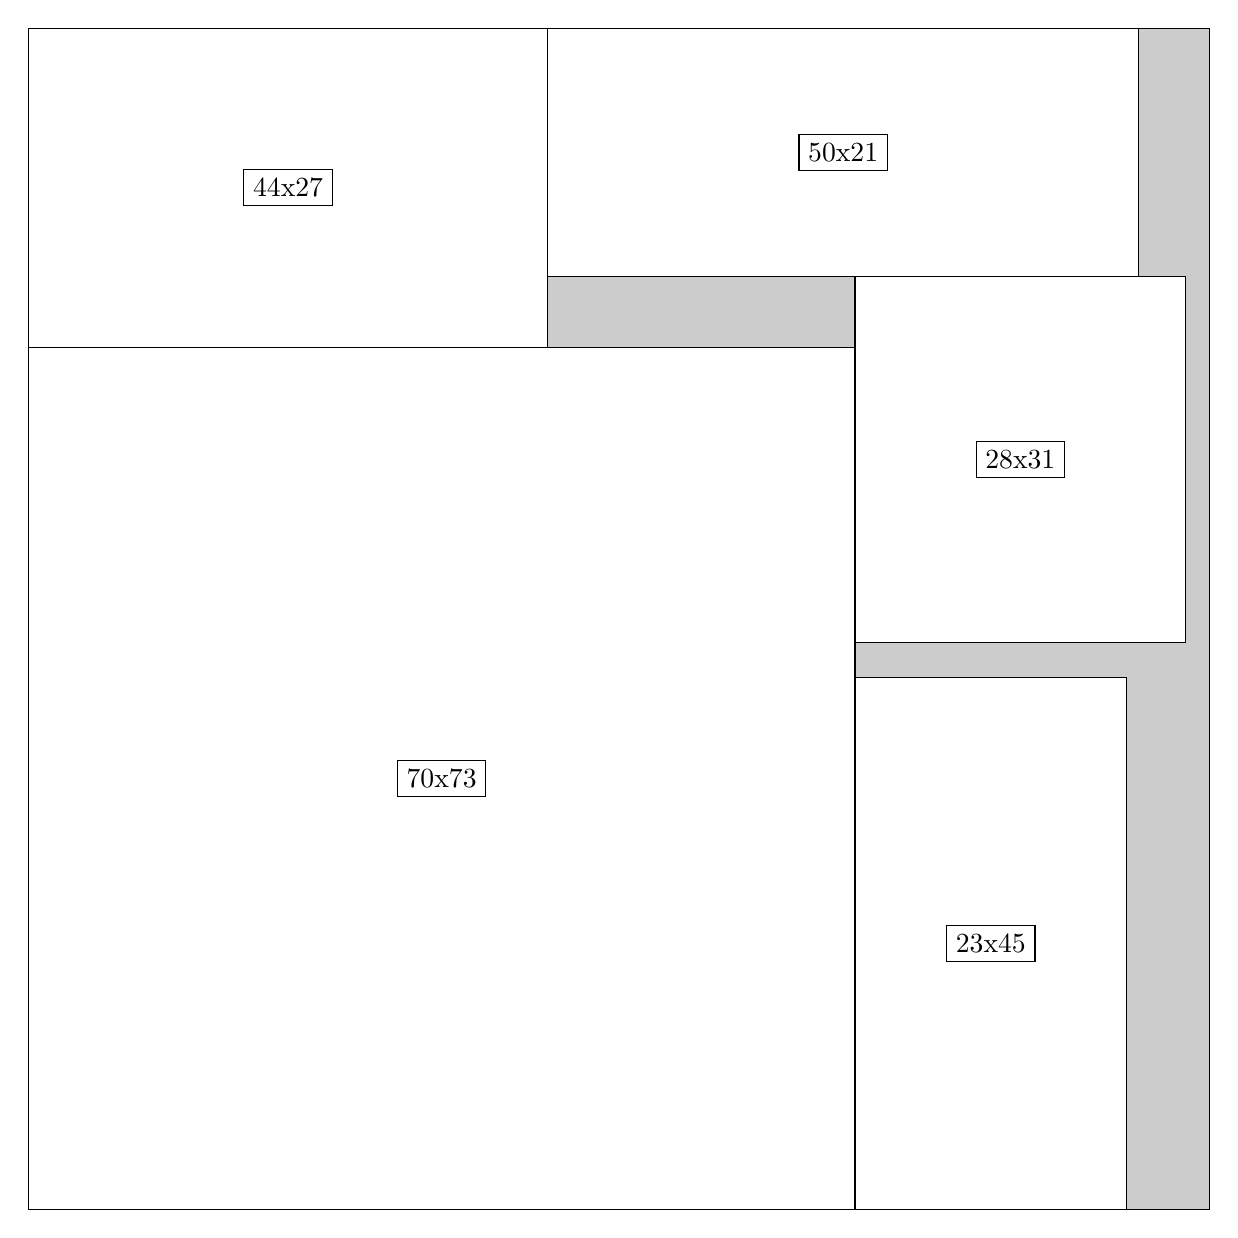
\begin{tikzpicture}[shorten >=1pt,scale=1.0,every node/.style={scale=1.0},->]
\tikzstyle{vertex}=[circle,fill=black!25,minimum size=14pt,inner sep=0pt]
\filldraw[fill=gray!40!white, draw=black] (0,0) rectangle (15.0,15.0);
\foreach \name/\x/\y/\w/\h in {70x73/0.0/0.0/10.5/10.95,44x27/0.0/10.95/6.6/4.05,50x21/6.6/11.85/7.5/3.15,23x45/10.5/0.0/3.4499999999999997/6.75,28x31/10.5/7.199999999999999/4.2/4.6499999999999995}
\filldraw[fill=white!40!white, draw=black] (\x,\y) rectangle node[draw] (\name) {\name} ++(\w,\h);
\end{tikzpicture}


w =70 , h =73 , x =0 , y =0 , v =5110
\par
w =44 , h =27 , x =0 , y =73 , v =1188
\par
w =50 , h =21 , x =44 , y =79 , v =1050
\par
w =23 , h =45 , x =70 , y =0 , v =1035
\par
w =28 , h =31 , x =70 , y =48 , v =868
\par
\newpage


\begin{tikzpicture}[shorten >=1pt,scale=1.0,every node/.style={scale=1.0},->]
\tikzstyle{vertex}=[circle,fill=black!25,minimum size=14pt,inner sep=0pt]
\filldraw[fill=gray!40!white, draw=black] (0,0) rectangle (15.0,15.0);
\foreach \name/\x/\y/\w/\h in {78x61/0.0/0.0/11.7/9.15,49x39/0.0/9.15/7.35/5.85,22x67/11.7/4.95/3.3/10.049999999999999,29x36/7.35/9.15/4.35/5.3999999999999995,22x33/11.7/0.0/3.3/4.95}
\filldraw[fill=white!40!white, draw=black] (\x,\y) rectangle node[draw] (\name) {\name} ++(\w,\h);
\end{tikzpicture}


w =78 , h =61 , x =0 , y =0 , v =4758
\par
w =49 , h =39 , x =0 , y =61 , v =1911
\par
w =22 , h =67 , x =78 , y =33 , v =1474
\par
w =29 , h =36 , x =49 , y =61 , v =1044
\par
w =22 , h =33 , x =78 , y =0 , v =726
\par
\newpage


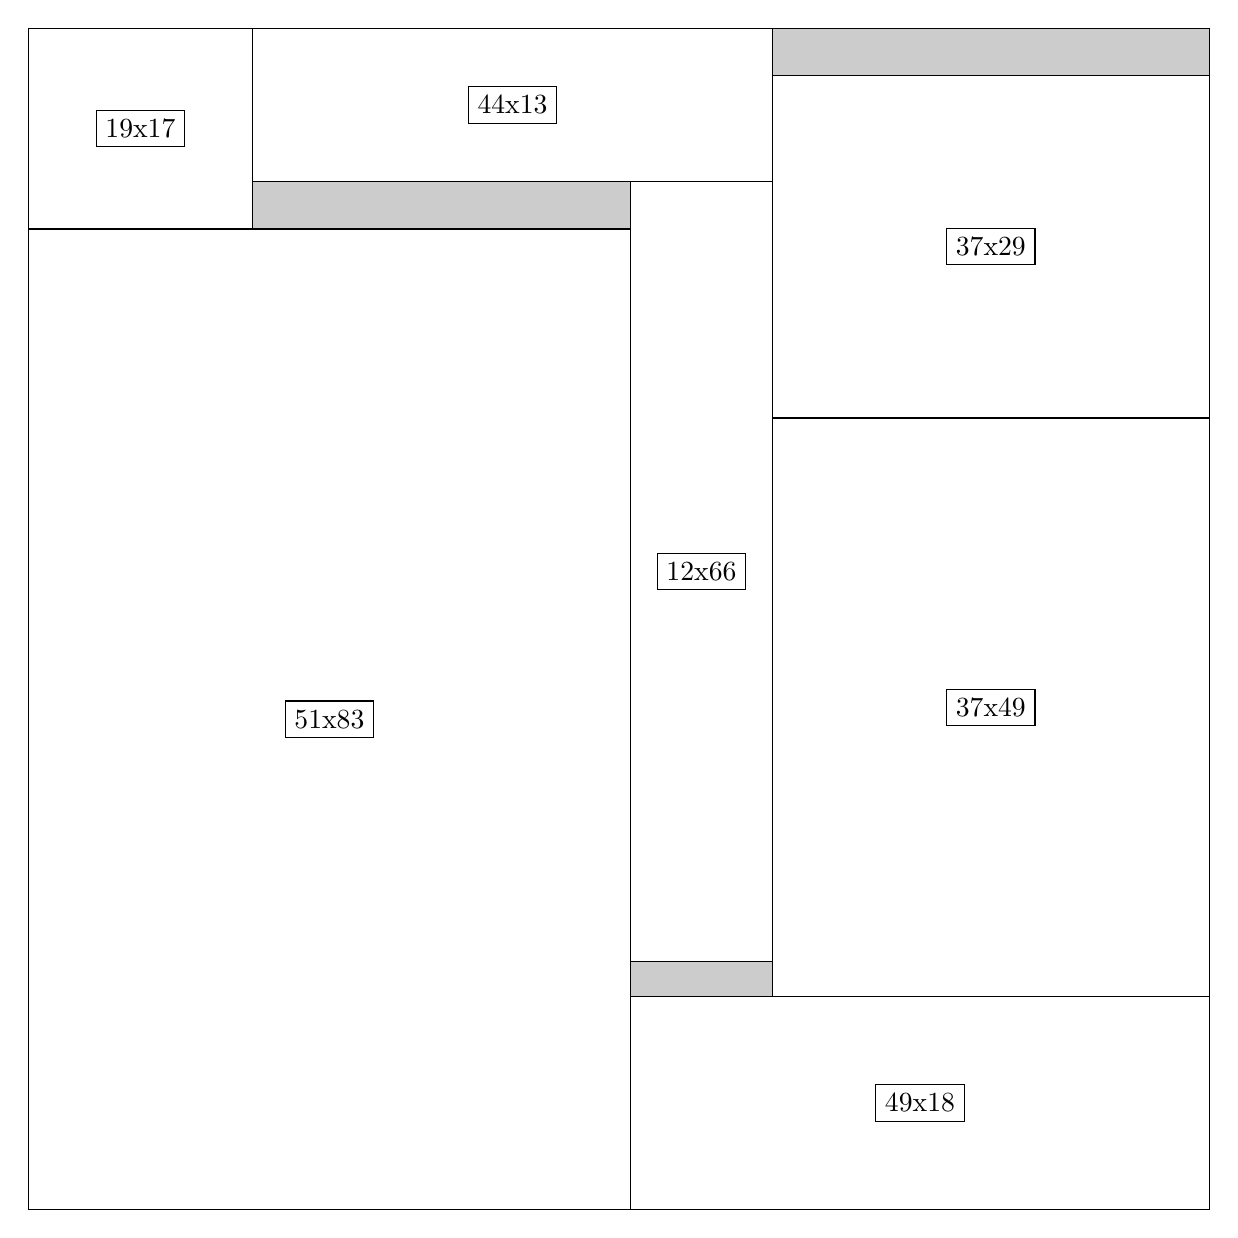
\begin{tikzpicture}[shorten >=1pt,scale=1.0,every node/.style={scale=1.0},->]
\tikzstyle{vertex}=[circle,fill=black!25,minimum size=14pt,inner sep=0pt]
\filldraw[fill=gray!40!white, draw=black] (0,0) rectangle (15.0,15.0);
\foreach \name/\x/\y/\w/\h in {51x83/0.0/0.0/7.6499999999999995/12.45,37x49/9.45/2.6999999999999997/5.55/7.35,37x29/9.45/10.049999999999999/5.55/4.35,19x17/0.0/12.45/2.85/2.55,12x66/7.6499999999999995/3.15/1.7999999999999998/9.9,44x13/2.85/13.049999999999999/6.6/1.95,49x18/7.6499999999999995/0.0/7.35/2.6999999999999997}
\filldraw[fill=white!40!white, draw=black] (\x,\y) rectangle node[draw] (\name) {\name} ++(\w,\h);
\end{tikzpicture}


w =51 , h =83 , x =0 , y =0 , v =4233
\par
w =37 , h =49 , x =63 , y =18 , v =1813
\par
w =37 , h =29 , x =63 , y =67 , v =1073
\par
w =19 , h =17 , x =0 , y =83 , v =323
\par
w =12 , h =66 , x =51 , y =21 , v =792
\par
w =44 , h =13 , x =19 , y =87 , v =572
\par
w =49 , h =18 , x =51 , y =0 , v =882
\par
\newpage


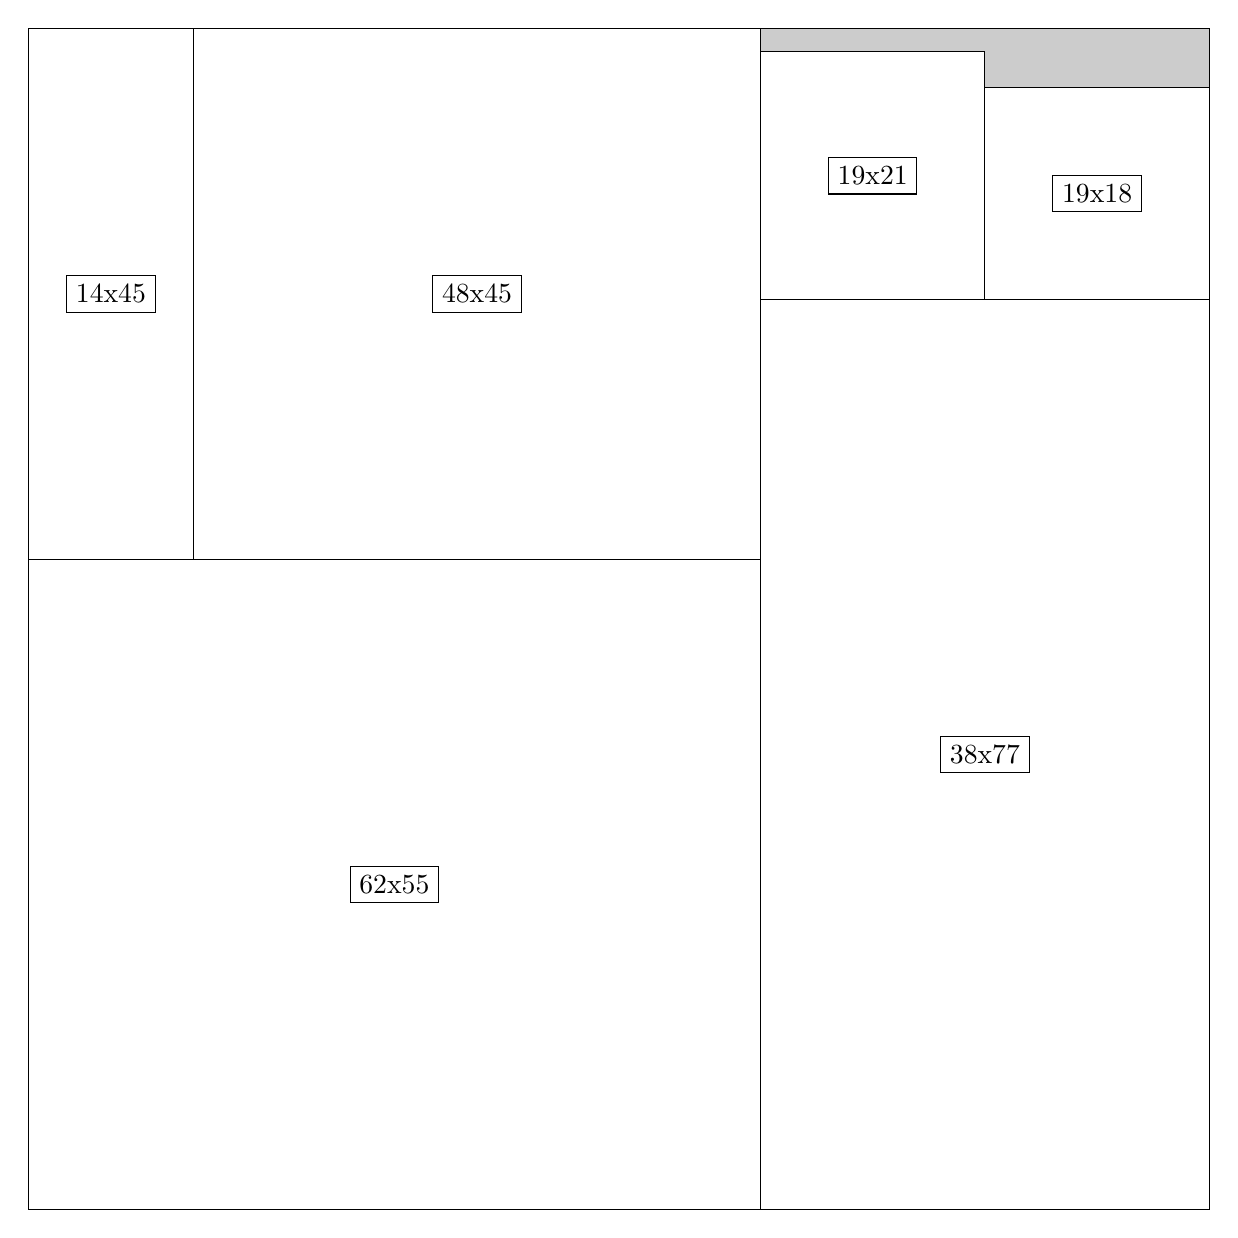
\begin{tikzpicture}[shorten >=1pt,scale=1.0,every node/.style={scale=1.0},->]
\tikzstyle{vertex}=[circle,fill=black!25,minimum size=14pt,inner sep=0pt]
\filldraw[fill=gray!40!white, draw=black] (0,0) rectangle (15.0,15.0);
\foreach \name/\x/\y/\w/\h in {38x77/9.299999999999999/0.0/5.7/11.549999999999999,14x45/0.0/8.25/2.1/6.75,48x45/2.1/8.25/7.199999999999999/6.75,62x55/0.0/0.0/9.299999999999999/8.25,19x21/9.299999999999999/11.549999999999999/2.85/3.15,19x18/12.15/11.549999999999999/2.85/2.6999999999999997}
\filldraw[fill=white!40!white, draw=black] (\x,\y) rectangle node[draw] (\name) {\name} ++(\w,\h);
\end{tikzpicture}


w =38 , h =77 , x =62 , y =0 , v =2926
\par
w =14 , h =45 , x =0 , y =55 , v =630
\par
w =48 , h =45 , x =14 , y =55 , v =2160
\par
w =62 , h =55 , x =0 , y =0 , v =3410
\par
w =19 , h =21 , x =62 , y =77 , v =399
\par
w =19 , h =18 , x =81 , y =77 , v =342
\par
\newpage


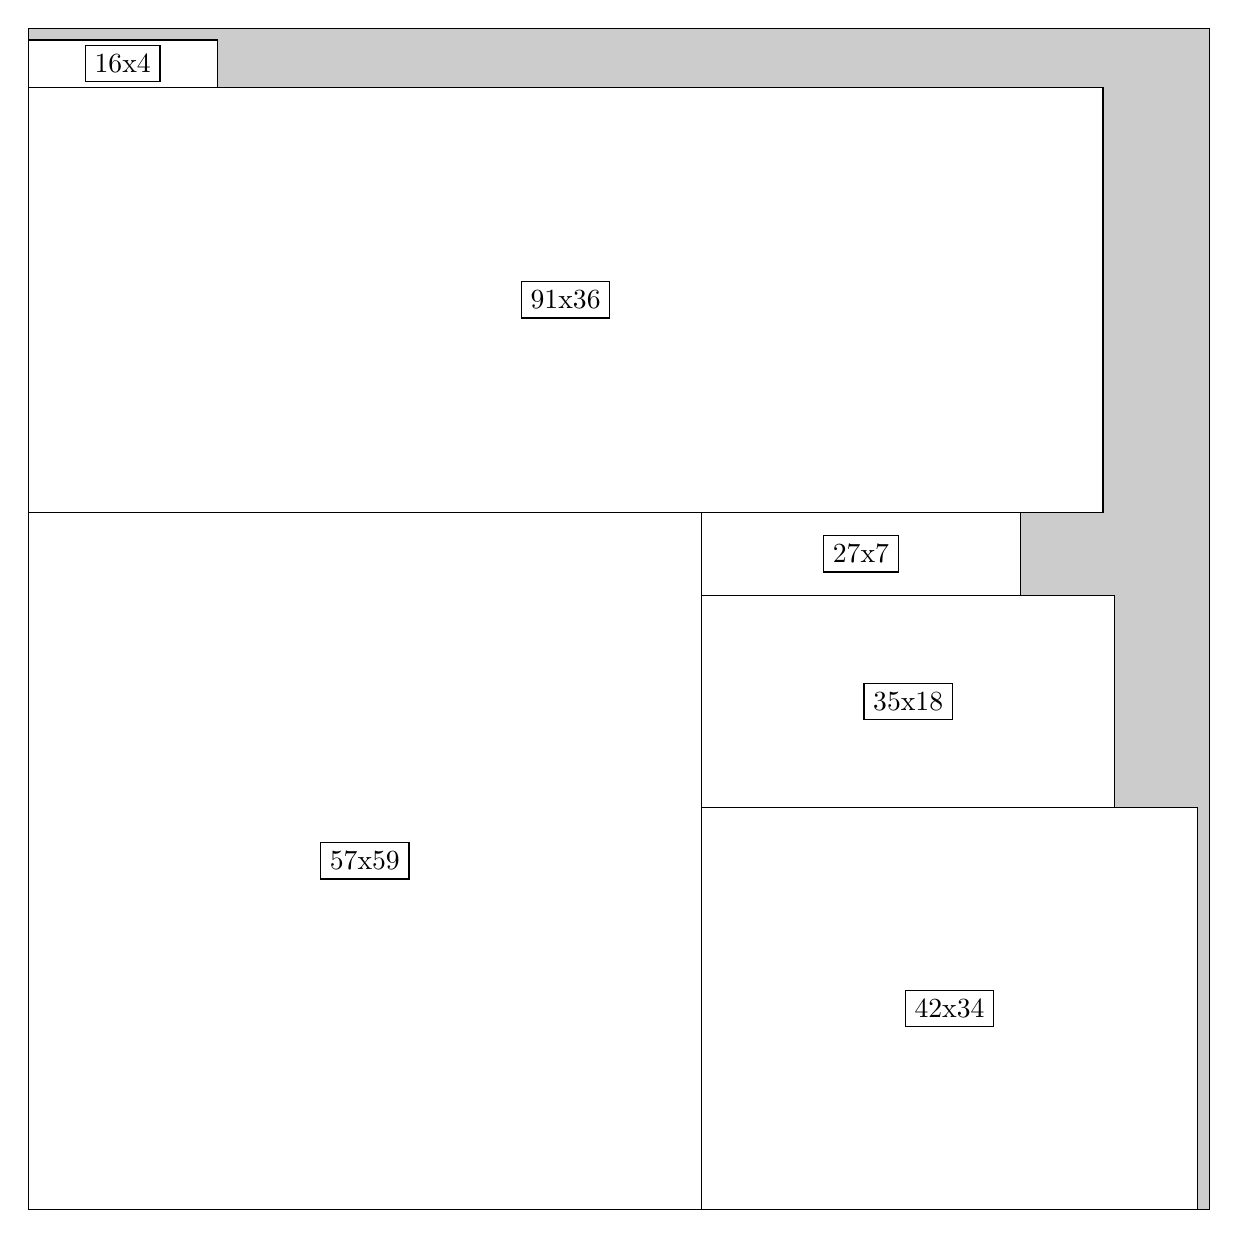
\begin{tikzpicture}[shorten >=1pt,scale=1.0,every node/.style={scale=1.0},->]
\tikzstyle{vertex}=[circle,fill=black!25,minimum size=14pt,inner sep=0pt]
\filldraw[fill=gray!40!white, draw=black] (0,0) rectangle (15.0,15.0);
\foreach \name/\x/\y/\w/\h in {57x59/0.0/0.0/8.549999999999999/8.85,91x36/0.0/8.85/13.65/5.3999999999999995,42x34/8.549999999999999/0.0/6.3/5.1,35x18/8.549999999999999/5.1/5.25/2.6999999999999997,27x7/8.549999999999999/7.8/4.05/1.05,16x4/0.0/14.25/2.4/0.6}
\filldraw[fill=white!40!white, draw=black] (\x,\y) rectangle node[draw] (\name) {\name} ++(\w,\h);
\end{tikzpicture}


w =57 , h =59 , x =0 , y =0 , v =3363
\par
w =91 , h =36 , x =0 , y =59 , v =3276
\par
w =42 , h =34 , x =57 , y =0 , v =1428
\par
w =35 , h =18 , x =57 , y =34 , v =630
\par
w =27 , h =7 , x =57 , y =52 , v =189
\par
w =16 , h =4 , x =0 , y =95 , v =64
\par
\newpage


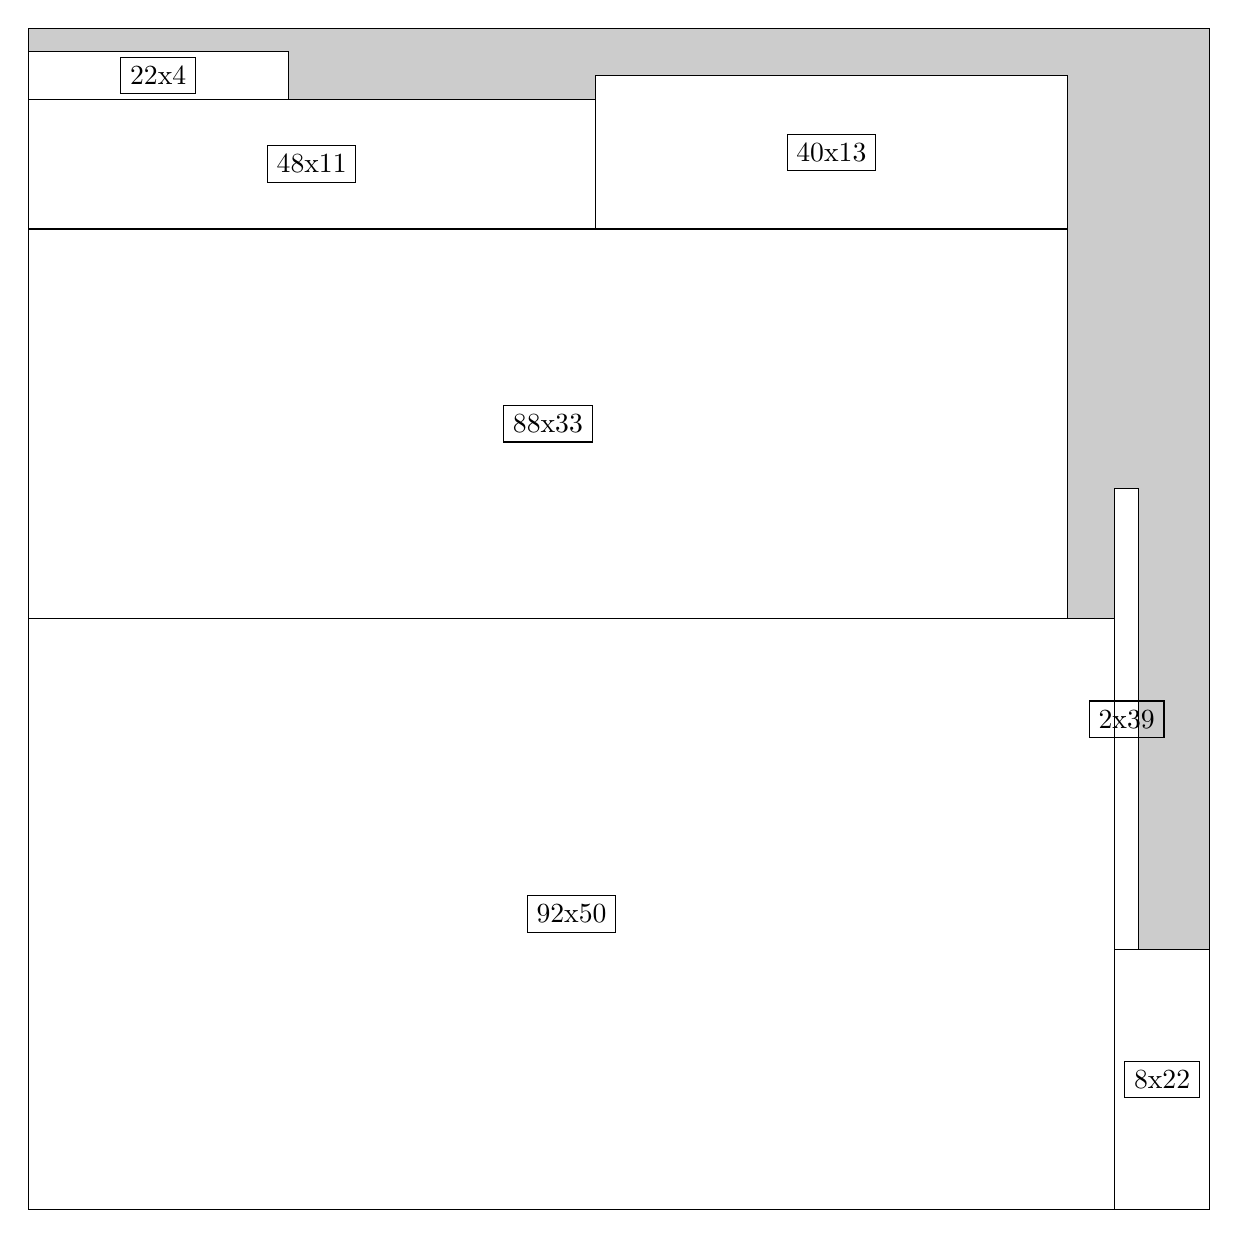
\begin{tikzpicture}[shorten >=1pt,scale=1.0,every node/.style={scale=1.0},->]
\tikzstyle{vertex}=[circle,fill=black!25,minimum size=14pt,inner sep=0pt]
\filldraw[fill=gray!40!white, draw=black] (0,0) rectangle (15.0,15.0);
\foreach \name/\x/\y/\w/\h in {92x50/0.0/0.0/13.799999999999999/7.5,88x33/0.0/7.5/13.2/4.95,48x11/0.0/12.45/7.199999999999999/1.65,40x13/7.199999999999999/12.45/6.0/1.95,8x22/13.799999999999999/0.0/1.2/3.3,22x4/0.0/14.1/3.3/0.6,2x39/13.799999999999999/3.3/0.3/5.85}
\filldraw[fill=white!40!white, draw=black] (\x,\y) rectangle node[draw] (\name) {\name} ++(\w,\h);
\end{tikzpicture}


w =92 , h =50 , x =0 , y =0 , v =4600
\par
w =88 , h =33 , x =0 , y =50 , v =2904
\par
w =48 , h =11 , x =0 , y =83 , v =528
\par
w =40 , h =13 , x =48 , y =83 , v =520
\par
w =8 , h =22 , x =92 , y =0 , v =176
\par
w =22 , h =4 , x =0 , y =94 , v =88
\par
w =2 , h =39 , x =92 , y =22 , v =78
\par
\newpage


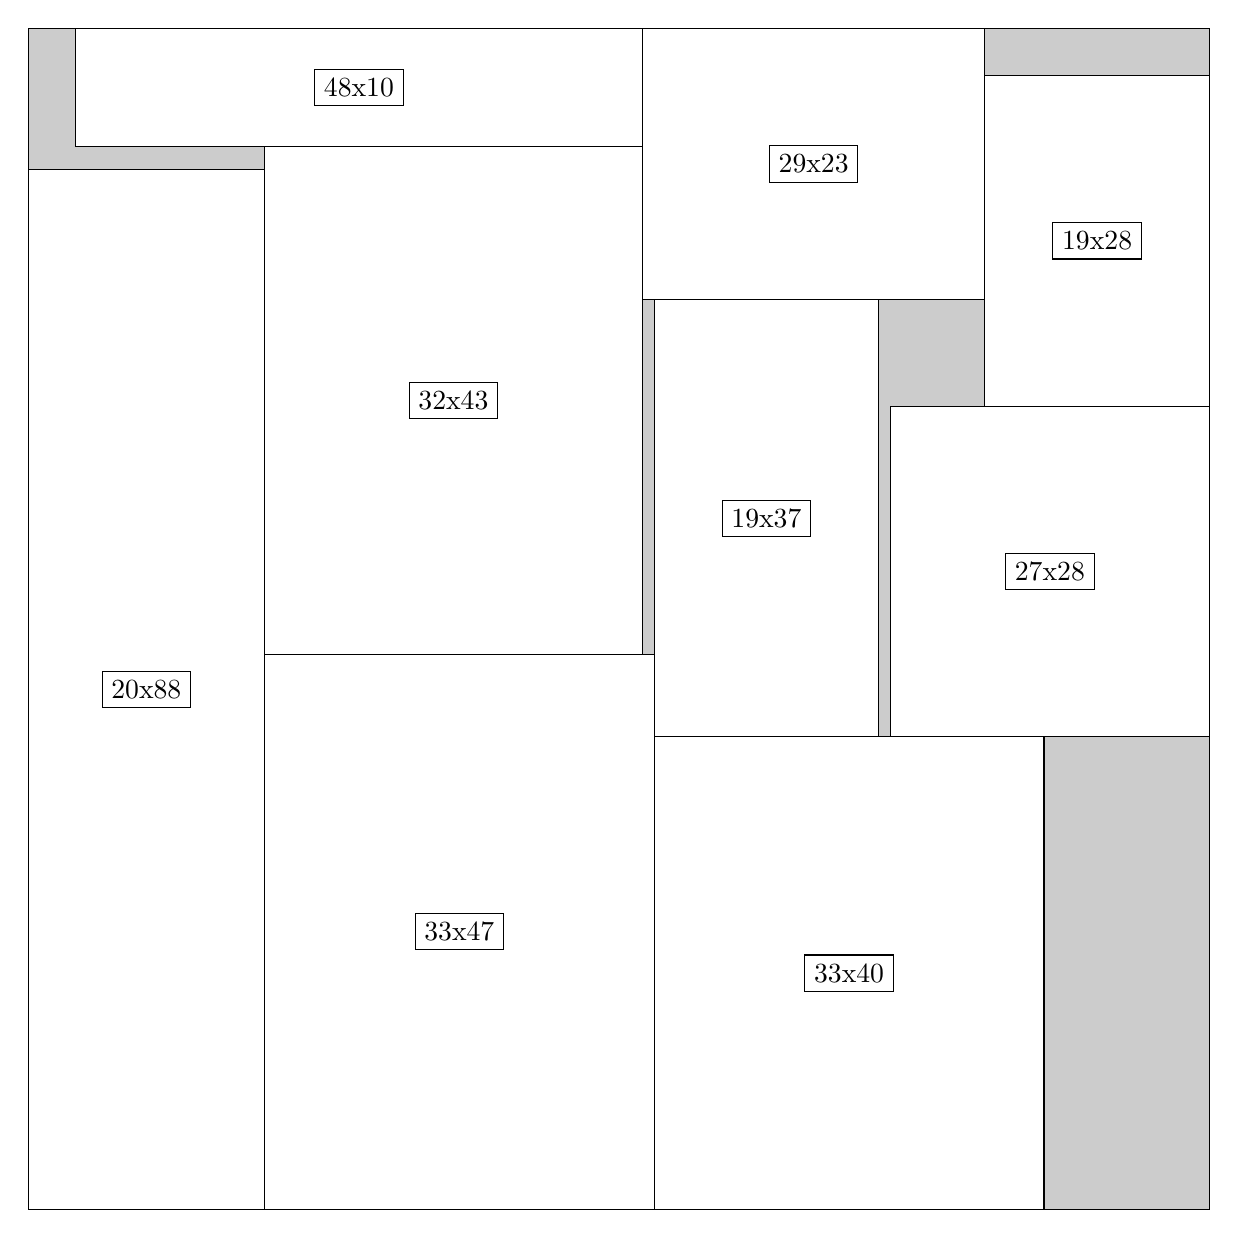
\begin{tikzpicture}[shorten >=1pt,scale=1.0,every node/.style={scale=1.0},->]
\tikzstyle{vertex}=[circle,fill=black!25,minimum size=14pt,inner sep=0pt]
\filldraw[fill=gray!40!white, draw=black] (0,0) rectangle (15.0,15.0);
\foreach \name/\x/\y/\w/\h in {20x88/0.0/0.0/3.0/13.2,33x47/3.0/0.0/4.95/7.05,32x43/3.0/7.05/4.8/6.45,33x40/7.949999999999999/0.0/4.95/6.0,27x28/10.95/6.0/4.05/4.2,19x37/7.949999999999999/6.0/2.85/5.55,29x23/7.8/11.549999999999999/4.35/3.4499999999999997,19x28/12.15/10.2/2.85/4.2,48x10/0.6/13.5/7.199999999999999/1.5}
\filldraw[fill=white!40!white, draw=black] (\x,\y) rectangle node[draw] (\name) {\name} ++(\w,\h);
\end{tikzpicture}


w =20 , h =88 , x =0 , y =0 , v =1760
\par
w =33 , h =47 , x =20 , y =0 , v =1551
\par
w =32 , h =43 , x =20 , y =47 , v =1376
\par
w =33 , h =40 , x =53 , y =0 , v =1320
\par
w =27 , h =28 , x =73 , y =40 , v =756
\par
w =19 , h =37 , x =53 , y =40 , v =703
\par
w =29 , h =23 , x =52 , y =77 , v =667
\par
w =19 , h =28 , x =81 , y =68 , v =532
\par
w =48 , h =10 , x =4 , y =90 , v =480
\par
\newpage


\end{document}